\documentclass[conference]{IEEEtran}
\IEEEoverridecommandlockouts
% The preceding line is only needed to identify funding in the first footnote. If that is unneeded, please comment it out.
\usepackage{cite}
\usepackage{amsmath,amssymb,amsfonts}
\usepackage{algorithmic}
\usepackage{graphicx}
\usepackage{textcomp}
\usepackage{xcolor}
\usepackage{url}
\usepackage[hidelinks]{hyperref}
\usepackage{booktabs}
\usepackage{float}



\def\BibTeX{{\rm B\kern-.05em{\sc i\kern-.025em b}\kern-.08em
    T\kern-.1667em\lower.7ex\hbox{E}\kern-.125emX}}
\begin{document}

\title{Detección de Deepfake en imágenes médicas\\}

\author{\IEEEauthorblockN{Juan Sebastián Ortiz Tangarife}
\IEEEauthorblockA{\textit{Ingeniería de sistemas} \\
\textit{Universidad de Antioquia}\\
Medellín, Colombia \\
juans.ortiz@udea.edu.co}
\and
\IEEEauthorblockN{David Agudelo Ochoa}
\IEEEauthorblockA{\textit{Ingeniería de sistemas} \\
\textit{Universidad de Antioquia}\\
Medellín, Colombia \\
david.agudeloo@udea.edu.co}
\and
\IEEEauthorblockN{Jose Franco Arroyave Cardona}
\IEEEauthorblockA{\textit{Ingeniería de sistemas} \\
\textit{Universidad de Antioquia}\\
Medellín, Colombia \\
franco.arroyave@udea.edu.co}

}

\maketitle

\section{Introducción}
\subsection{Contexto del problema}

En los últimos años, el desarrollo de redes generativas adversariales (GANs) y otras técnicas avanzadas de inteligencia artificial ha permitido la creación de deepfakes (imágenes, audios o videos manipulados de manera que simulan ser reales). En este contexto, el término "deepfake" se refiere a contenido generado artificialmente, a menudo con el objetivo de engañar o desinformar. Aunque estos avances han permitido mejoras en muchas áreas, también han planteado serios desafíos, especialmente en campos donde la precisión y la veracidad son críticas, como en el ámbito médico.

En el campo de imágenes médicas, las tomografías computarizadas (CT), resonancias magnéticas (MRI) y otras imágenes diagnósticas son fundamentales para el diagnóstico y tratamiento de enfermedades. Las manipulaciones de estas imágenes a través de técnicas de deepfake pueden ser extremadamente peligrosas, ya que pueden alterar los diagnósticos médicos, llevando a decisiones incorrectas y perjudicando el bienestar de los pacientes. Por ejemplo, una imagen manipulada de una radiografía podría hacer que un tumor visible sea invisible, o que un área sana sea interpretada erróneamente como problemática.

El objetivo principal de este proyecto es desarrollar una solución automatizada basada en Machine Learning para la detección de imágenes médicas manipuladas. Esto permitiría a los profesionales de la salud contar con una herramienta que los ayude a identificar si una imagen ha sido alterada de alguna manera, lo que contribuiría a preservar la confiabilidad de los diagnósticos médicos.

La implementación de una solución de este tipo es crucial en un contexto donde la información médica es cada vez más digitalizada y accesible en plataformas online, lo que aumenta la probabilidad de que imágenes manipuladas circulen. La detección eficiente de estos deepfakes en imágenes médicas no solo ayudaría a garantizar diagnósticos correctos, sino también a mejorar la seguridad y la confianza en el uso de imágenes digitales para la toma de decisiones médicas.

\subsection{Composición de la base de datos}

La base de datos utilizada se llama Deepfakes: Medical Image Tamper Detection (CT-GAN). Este conjunto de datos fue creado para estudiar la manipulación de imágenes médicas mediante técnicas de aprendizaje profundo (deep learning), específicamente en escaneos 3D de tomografía computarizada (CT) de los pulmones\cite{uci2020deepfakes}.
Se utilizaron redes generativas adversarias (GANs) para alterar los escaneos, ya sea insertando cáncer falso (lesiones falsas) o eliminando cáncer real, simulando un ataque malicioso. El objetivo del dataset es permitir el desarrollo y evaluación de técnicas de detección de imágenes médicas alteradas (deepfakes médicos).

\paragraph{Contenido del conjunto de datos}

\begin{itemize}
    \item 100 estudios de tomografía computarizada (CT scans) de tórax.
    \item Cada escaneo contiene múltiples cortes (slices) de 512x512 píxeles, formando un volumen 3D.
    \item Los datos están en formato DICOM, el estándar médico para imágenes.
\end{itemize}

\paragraph{Clasificación de los escaneos}
Cada volumen está etiquetado según el tipo de manipulación presente:

\begin{itemize}
    \item \textbf{True-Benign(TB)}: Zona sin cáncer, no manipulada.
    \item \textbf{True-Malignant(TM)}: Zona con cáncer real, no manipulada.
    \item \textbf{False-Benign(FB)}: Cáncer real que fue eliminado con deepfake (engañosamente parece sano).
    \item \textbf{False-Malignant(FM)}: Se añadió un cáncer falso con deepfake (engañosamente parece enfermo).
\end{itemize}

\paragraph{Número de muestras}
Cada muestra corresponde a una imagen médica individual en formato \texttt{.dcm} (DICOM). Las imágenes están organizadas por paciente, donde cada carpeta representa a un paciente y contiene múltiples cortes (slices) de su estudio médico. El número total de imágenes es el siguiente:

\begin{itemize}
    \item \textbf{Experiment 1 - Blind}: 17,457 imágenes
    \item \textbf{Experiment 2 - Open}: 5,296 imágenes
    \item \textbf{Total}: 22,753 imágenes
\end{itemize}

\paragraph{Explicación experimentos}
La base de datos está dividida en dos experimentos: Experiment 1 - Blind y Experiment 2 - Open, estos se diferencian en el nivel de información disponible sobre las manipulaciones.

\begin{itemize}
\item \textbf{Experiment 1 - Blind:} En este experimento, las anotaciones de las regiones manipuladas no fueron utilizadas durante el entrenamiento. Este enfoque simula un escenario más realista, donde las manipulaciones son desconocidas de antemano, y se espera que el modelo aprenda a detectarlas sin depender de etiquetas precisas sobre la ubicación del deepfake.
\item \textbf{Experiment 2 - Open:} En este caso, sí se proporcionaron anotaciones explícitas de las regiones manipuladas durante el entrenamiento. El modelo conocía durante el proceso de aprendizaje qué partes de las imágenes estaban alteradas. Este enfoque permite una supervisión más precisa, y se espera que los modelos logren un desempeño más alto al tener acceso directo a la "verdad" respecto a las alteraciones en cada imagen.
\end{itemize}


\paragraph{Anotaciones}
Cada experimento incluye un archivo \texttt{CSV} con anotaciones que indican regiones alteradas dentro de las imágenes. Cada fila en estos archivos representa una anotación, es decir, una posible manipulación en una ubicación específica de una imagen.

\begin{itemize}
    \item \textbf{Experiment 1 - Blind}: 133 anotaciones
    \item \textbf{Experiment 2 - Open}: 36 anotaciones
    \item \textbf{Total}: 169 anotaciones
\end{itemize}

Las variables presentes en ambos archivos son:

\begin{itemize}
    \item \textbf{type}: Tipo de manipulación (por ejemplo, \texttt{FB}).
    \item \textbf{uuid}: Identificador único del paciente.
    \item \textbf{slice}: Número de corte de la imagen donde se encuentra la anotación.
    \item \textbf{x}, \textbf{y}: Coordenadas dentro del corte donde se localiza la alteración. Esto brinda la posibilidad de abordar el problema como una tarea de localización de regiones alteradas, usando técnicas como detección de objetos o segmentación.
\end{itemize}


\paragraph{Datos faltantes}
Tras una revisión completa, no se encontraron datos faltantes en los datasets. 

\paragraph{Codificación de variables}

Las variables del conjunto de datos se clasifican como sigue:

\begin{itemize}
    \item \textbf{Variables categóricas}:
        \begin{itemize}
            \item \texttt{type}
        \end{itemize}
    \item \textbf{Variables numéricas}:
        \begin{itemize}
            \item \texttt{uuid}, \texttt{slice}, \texttt{x}, \texttt{y}
        \end{itemize}
\end{itemize}

\subsection{Paradigma de aprendizaje}

El problema de detección de deepfakes en imágenes médicas se aborda como una tarea de clasificación binaria supervisada. Cada imagen se etiqueta como alterada (es decir, manipulada mediante técnicas de deepfake) o no alterada (imagen original sin modificaciones). De esta manera, el objetivo del modelo es aprender a distinguir patrones que permitan identificar si una imagen ha sido manipulada o no.
Dado que el objetivo no es identificar el tipo de manipulación ni su ubicación exacta, sino simplemente determinar si existe o no una alteración, este enfoque binario permite simplificar el problema y centrarse en detectar patrones globales de manipulación.

El conjunto de datos está desbalanceado, ya que hay muchas más imágenes manipuladas (FB, FM) que originales (TM, TB). Para reducir un poco ese desbalance, se trabajó principalmente sobre la clase TB, duplicando las muestras y generando cortes adicionales alrededor del corte original. Esto se hizo desplazando el valor del corte (slice) hacia adelante y hacia atrás, como si se tomaran imágenes vecinas dentro del mismo estudio. Así se logra aumentar la cantidad de ejemplos TB sin alterar su clase.


\section{Estado del Arte}

Los autores Yetiş y Çeçen se centraron en detectar si las imágenes médicas habían sido manipuladas~\cite{yetis2024}, es decir, si correspondían a un \textit{deepfake}, abordando el problema mediante un enfoque de clasificación binaria supervisada. Aunque el conjunto de datos contiene múltiples instancias por tomografía, cada uno de los cortes fue tratado como una muestra completa e independiente. El problema se abordó utilizando distintas variantes de la familia de modelos YOLO (You Only Look Once), especializada en la detección de objetos en imágenes, y cuya aplicación ha demostrado ser relevante en escenarios relacionados con \textit{deepfakes} médicos.

De manera similar, Solaiyappan y Wen también trataron el problema de detección de \textit{deepfakes} médicos como una tarea de clasificación binaria supervisada~\cite{solaiyappan2022}. En este caso, se exploraron tanto modelos convencionales como modelos de aprendizaje profundo. Entre las técnicas utilizadas se incluyeron clasificadores clásicos como SVM, Random Forest y árboles de decisión, así como redes convolucionales preentrenadas como ResNet, VGG y DenseNet, adaptadas posteriormente mediante \textit{fine-tuning}. Al igual que en el trabajo anterior, cada corte 2D fue tratado de forma independiente, sin modelar la secuencia 3D completa.

Sharafudeen y Chandra~\cite{sharafudeen2022} propusieron una arquitectura basada en redes neuronales convolucionales tridimensionales (3D-CNN) para abordar el mismo problema, con la ventaja de preservar la información espacial y contextual del volumen completo de la tomografía. El modelo fue entrenado con un 80\% de los datos, validado con un 10\%, y evaluado con el 10\% restante. La métrica principal reportada fue la exactitud (\textit{accuracy}), alcanzando un desempeño cercano al 98\%.

Por su parte, Albahli y Nawaz~\cite{albahli2023} propusieron una arquitectura híbrida llamada MedNet, que combina capas convolucionales con un enfoque de red neuronal multicapa para la clasificación final. A diferencia de los trabajos anteriores, utilizaron validación cruzada como método de evaluación y reportaron múltiples métricas: AUC, F1-score, precisión y exactitud. Sus resultados reflejaron un rendimiento robusto, con valores de exactitud superiores al 99\%.

Para la validación de los resultados, los autores Yetiş y Çeçen realizaron una partición del conjunto de datos en 80\% para entrenamiento y 20\% para prueba. No se menciona el uso de validación cruzada. Por su parte, Solaiyappan y Wen también emplearon una partición de los datos en entrenamiento y prueba, aunque no se especifica la proporción exacta ni el uso de técnicas de validación cruzada. En los otros dos estudios, sí se especifican claramente las estrategias de validación.

El rendimiento de los modelos del primer estudio~\cite{yetis2024} se evaluó mediante métricas estándar en tareas de detección de objetos: precisión (\textit{precision}), recobrado (\textit{recall}) y media de precisión promedio (\textit{mAP}). Estas métricas se calculan en función de la Intersección sobre la Unión (IoU), que mide el grado de coincidencia entre las cajas predichas y las reales en la detección. En el segundo y tercer estudio~\cite{solaiyappan2022, sharafudeen2022}, las métricas empleadas se centraron en la exactitud (\textit{accuracy}), con resultados que mostraron valores casi perfectos en los mejores modelos de \textit{deep learning} utilizados. En el último trabajo~\cite{albahli2023}, se utilizaron métricas como la AUC y el F1-score, lo que permitió una evaluación más completa delrendimiento de los modelos.

Según el análisis de resultados, el modelo YOLOv5 su fue el más eficaz para la detección de manipulaciones en imágenes médicas del tipo CT, alcanzando un \textit{recall} de 0{,}997 y un \textit{mAP} superior a 0{,}931~\cite{yetis2024}. Por otro lado, en el trabajo de Solaiyappan y Wen, los modelos basados en redes profundas como ResNet50 y DenseNet121 lograron desempeños notables, con exactitudes cercanas al 100\%~\cite{solaiyappan2022}. De manera similar, los modelos propuestos por Sharafudeen y Chandra~\cite{sharafudeen2022} y por Albahli y Nawaz~\cite{albahli2023} demostraron una alta capacidad de generalización, con exactitudes mayores al 98\% y métricas adicionales que respaldan la solidez de sus enfoques.



\begin{table}[ht]
\centering
\caption{Comparación de artículos sobre detección de deepfakes médicos}
\begin{tabular}{p{1.3cm} p{1cm} p{1cm} p{1.2cm} p{1cm} p{1cm}}
\toprule
\textbf{Artículo} & \textbf{Modelo usado} & \textbf{Tipo de dato} & \textbf{Validación} & \textbf{Métricas} & \textbf{Accuracy / mAP} \\
\midrule
Yetiş y Çeçen (2024) & YOLOv5 & Cortes 2D independientes & 80/20 & mAP, Recall, Precision & mAP $>$ 0.931 \\
\midrule
Solaiyappan y Wen (2022) & ResNet50, SVM & Cortes 2D & No especificada & Accuracy & $\approx$ 100\% \\
\midrule
Sharafudeen y Chandra (2022) & 3D-CNN & Volumen 3D & 80/10/10 & Accuracy & $\approx$ 98\% \\
\midrule
Albahli y Nawaz (2023) & MedNet híbrido & CT-GAN & Validación cruzada & AUC, F1, Accuracy & $>$ 99\% \\
\bottomrule
\end{tabular}
\label{tab:comparacion-articulos}
\end{table}





\section{Entrenamiento y Evaluación de Modelos}

\subsection{Preprocesamiento y Aumento de Datos}

El conjunto de datos fue procesado en varias etapas para mejorar la calidad y balance de las clases antes del entrenamiento:

\begin{itemize}
    \item \textbf{Etiquetado}: Se asignó \texttt{label=1} a muestras cuyo campo \texttt{type} inicia con \texttt{F} (FB, FM), y \texttt{label=0} a las que inician con \texttt{T} (TB, TM). Así queda explícito que lo que se busca es encontrar los casos de deepfake.
    \item \textbf{Filtrado}: Se mantuvieron todas las muestras no pertenecientes a la categoría TB y, para las muestras TB, se eliminó duplicidad por identificador \texttt{uuid}, conservando una única entrada por estudio.
    \item \textbf{Aumento con cortes vecinos}: Se generaron muestras adicionales desplazando el número de corte (\texttt{slice}) hacia adelante y hacia atrás en 5 (\texttt{+st} y \texttt{-st}), creando así imágenes de cortes vecinos. Las nuevas muestras fueron marcadas con \texttt{generated=1}.
    \item \textbf{Transformaciones aleatorias}: Sobre las muestras generadas, se aplicaron rotaciones leves, escalado, y adición de ruido gaussiano y uniforme, con el fin de incrementar la variabilidad y robustez del conjunto.
    \item \textbf{Conversión DICOM a PNG}: Cada archivo \texttt{.dcm} se transformó mediante ajuste de ventana para mejorar contraste, y luego se exportó a formato PNG, más adecuado para procesar en redes neuronales.
\end{itemize}

Este flujo permitió aumentar significativamente la cantidad original de muestras como se observa en la Tabla~\ref{tab:dataset}. Además de esto, el flujo anterior permitió  aportar mayor variabilidad, mejorando así la capacidad de generalización de los modelos que se entrenaron.

\begin{table}[h]
\centering
\caption{Tamaño del conjunto de datos y distribución de clases}
\begin{tabular}{lc}
\toprule
\textbf{Característica} & \textbf{Valor} \\
\midrule
Tamaño original & (158, 6) \\
Tamaño final & (474, 7) \\
Cantidad de muestras clase 1 & 339 \\
Cantidad de muestras clase 0 & 135 \\
\bottomrule
\end{tabular}
\label{tab:dataset}
\end{table}



\subsection{Extracción de Características}

El proceso de extracción de características se diseñó para convertir las imágenes médicas, previamente transformadas a formato PNG, en un conjunto de datos tabular (\texttt{X}) que pudiera ser empleado en la fase de entrenamiento y evaluación de modelos de clasificación. 

Se optó por representar las imágenes mediante vectores de características para garantizar que todos los modelos pudieran ser comparados en igualdad de condiciones, evitando que algunos recibieran directamente las imágenes mientras que otros solo trabajaran con descriptores tabulares.

En primer lugar, se procesaron todas las imágenes del conjunto utilizando descriptores clásicos de textura ampliamente utilizados en la literatura, en particular: Gray Level Co-occurrence Matrix (GLCM) y Local Binary Patterns (LBP). Cada imagen fue leída en escala de grises y, para cada una, se calcularon tanto los histogramas normalizados de LBP como las estadísticas derivadas de GLCM (contraste, homogeneidad, energía, correlación y entropía).

Durante el desarrollo experimental, se exploraron inicialmente diversas configuraciones:
\begin{itemize}
    \item Extracción de características únicamente con LBP.
    \item Extracción de características únicamente con GLCM.
    \item Extracción de características únicamente con Histogram of Oriented Gradients (HOG).
    \item Extracción de características mediante una red profunda ResNet-18 preentrenada en ImageNet, empleando el vector generado por la penúltima capa como representación de la imagen.
\end{itemize}

Tras varios intentos y evaluaciones preliminares, se observó que la combinación de GLCM y LBP proporcionaba mejores resultados de clasificación que el uso individual de cada descriptor mencionado anteriormente. Por tanto, la versión final del dataset se construyó uniendo las características extraídas con GLCM y LBP, manteniendo así un equilibrio entre complejidad computacional y capacidad de discriminación.

El DataFrame resultante se compone de las siguientes partes:
\begin{itemize}
    \item \textbf{X}: matriz de características con forma $(n\_muestras, n\_características)$.
    \item \textbf{y}: vector de etiquetas asociadas a cada muestra.
    \item \textbf{groups}: vector con los identificadores únicos (\texttt{uuid}), útil para estrategias de validación cruzada agrupada (por paciente o estudio).
\end{itemize}
La dimensión de cada uno de estos puede ser observado en la Tabla~\ref{tab:final_dimensions}.

\begin{table}[h]
\centering
\caption{Dimensiones de los conjuntos obtenidos tras la extracción de características}
\begin{tabular}{lc}
\toprule
\textbf{Conjunto} & \textbf{Dimensión} \\
\midrule
\textit{X} & (474, 30) \\
\textit{y} & (474,) \\
\textit{groups} & (474,) \\
\bottomrule
\end{tabular}
\label{tab:final_dimensions}
\end{table}

Finalmente, los datos fueron almacenados tanto en formato comprimido \texttt{.npz} como en formato \texttt{.pkl}, permitiendo una carga eficiente para la siguiente fase.








\subsection{Selección y Reducción de Características}

Con el fin de reducir la dimensionalidad del conjunto de datos, mejorar la interpretabilidad y facilitar el entrenamiento de los modelos, se aplicaron y compararon tres estrategias diferentes: selección por filtro estadístico, selección recursiva con validación supervisada y reducción no supervisada mediante componentes principales.

\begin{itemize}
    \item \textbf{Filtro estadístico (SelectKBest):} se calculó el estadístico ANOVA F-score para cada característica extraída (GLCM, LBP, etc.). Las características se ordenaron según su importancia estadística y se conservaron únicamente las $k=15$ con mayor puntuación como se muestra en la Figura~\ref{fig:anova}. Esta técnica permite identificar aquellas variables que presentan mayor discriminación respecto a las etiquetas de clase.

    \begin{figure}[htbp]
    \centering
    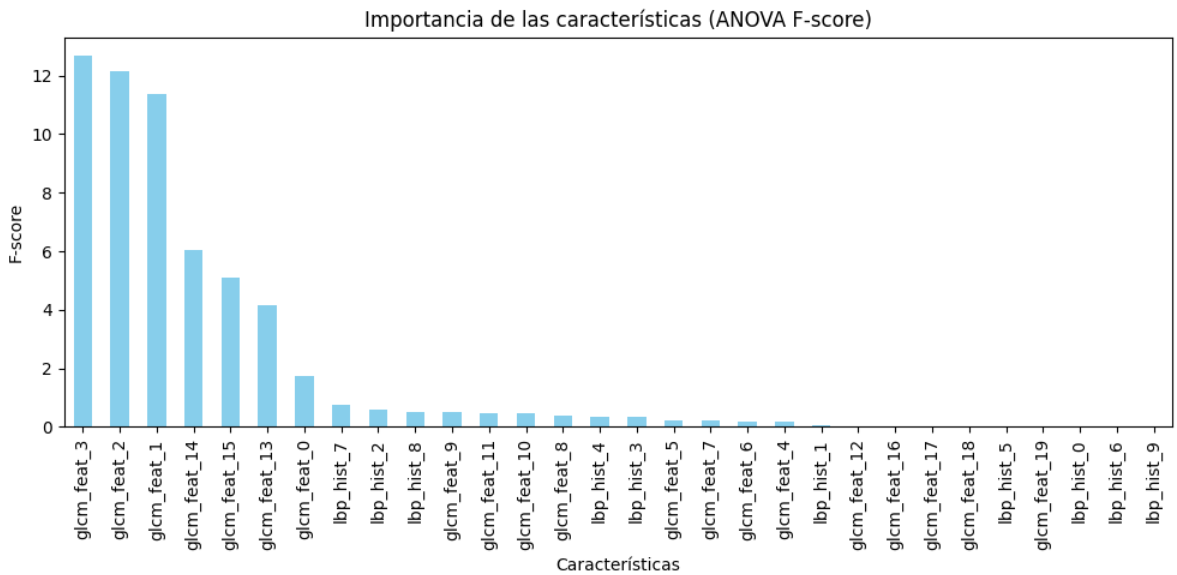
\includegraphics[width=0.5\textwidth]{images/f scores.png}
    \caption{ANOVA F-SCORE}
    \label{fig:anova}
    \end{figure}
    
    \item \textbf{Selección recursiva con Random Forest (RFE):} se entrenó un modelo Random Forest sobre los datos y se aplicó RFE (\emph{Recursive Feature Elimination}) para seleccionar iterativamente las $15$ características más relevantes para la clasificación como se muestra en la Figura~\ref{fig:rfe}. Posteriormente, el modelo se reentrenó únicamente con esas características seleccionadas, obteniendo además la importancia de cada variable y la curva ROC para evaluar el desempeño.

    \begin{figure}[htbp]
    \centering
    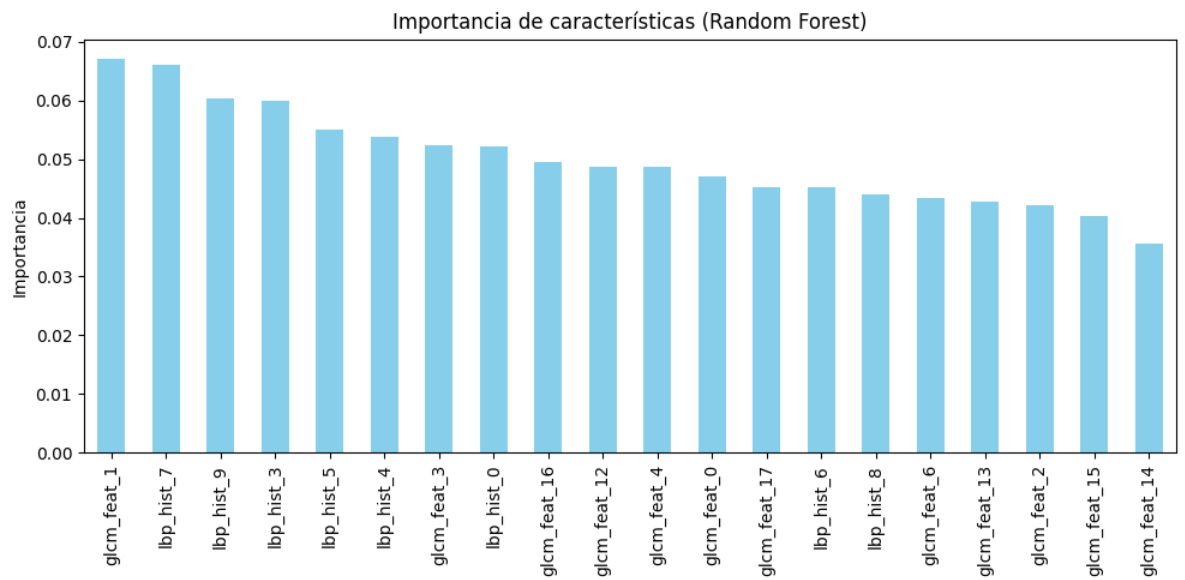
\includegraphics[width=0.5\textwidth]{images/rf.png}
    \caption{RANDOM FOREST}
    \label{fig:rfe}
    \end{figure}
    


    \item \textbf{Reducción no supervisada (PCA):} se aplicó \emph{Principal Component Analysis} para proyectar los datos originales en un subespacio de $15$ componentes principales, como se muestra en la Figura~\ref{fig:pca}. Se calculó y graficó la varianza explicada por cada componente y la varianza acumulada, lo que permite visualizar el grado en que la estructura de los datos puede representarse en un espacio de menor dimensión. Tras este análisis, se observó que la mayor parte de la varianza queda concentrada en el primer componente principal, lo que indica una alta dependencia y correlación entre las características originales; en otras palabras, muchas de ellas contienen información redundante.

    
    \begin{figure}[htbp]
    \centering
    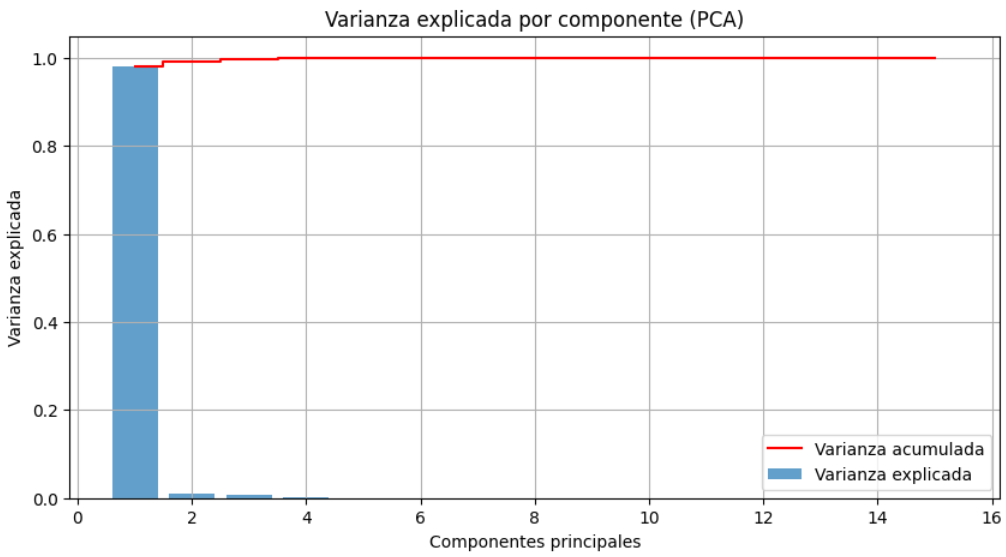
\includegraphics[width=0.5\textwidth]{images/pca.png}
    \caption{Varianza explicada y acumulada tras aplicar PCA}
    \label{fig:pca}
    \end{figure}
    \end{itemize}

Cada técnica genera un nuevo conjunto de datos reducido, que puede evaluarse posteriormente en los modelos de clasificación para determinar cuál estrategia conserva mejor la información relevante para la tarea de detección.























\subsection{Modelos implementados}

Se probaron los siguientes algoritmos:
\begin{itemize}
    \item Regresión logística
    \item K-Nearest Neighbors (KNN)
    \item Random Forest
    \item Support Vector Machine (SVM)
    \item Red neuronal multicapa (MLP)
\end{itemize}


\subsection{Entrenamiento}


Los datos se dividieron mediante 2 splits de la siguiente forma. 
\begin{itemize}
    \item Primer split: 90\% \textit{Train+Validation}, 10\% \textit{Test}.
    \item Segundo split: 80\% \textit{Train}, 20\% \textit{Validation} dentro del 90\% original.
\end{itemize}


Obteniendo así, train (339 muestras), val (87) y test (48) preservando la proporción de clases por paciente. Todos los modelos usaron escalado estándar y se optimizaron mediante búsqueda en grilla con validación cruzada usando Group K-folds (5-folds).

A continuación se presentan los resultados obtenidos para cada uno de los modelos:
\newline
\newline

\subsubsection{Regresión Logística}

\textbf{Mejor combinación de hiperparámetros:} 

\text{C=0.01, penalty=l2, solver=lbfgs}

\textbf{Mejor F1-score (CV):} 0.8341 

\textbf{Accuracy medio (CV):} 0.7200 

\textbf{Recall medio (CV):} 0.9933

\begin{table}[htbp]
\centering
\caption{Reporte de clasificación en entrenamiento (Regresión Logística)}
\begin{tabular}{lcccc}
\toprule
 & Precision & Recall & F1-score & Support \\
\midrule
Real & 0.77 & 0.06 & 0.11 & 165 \\
Fake & 0.74 & 0.99 & 0.85 & 435 \\
\midrule
Accuracy & & & 0.74 & 600 \\
Macro avg & 0.75 & 0.53 & 0.48 & 600 \\
Weighted avg & 0.75 & 0.74 & 0.64 & 600 \\
\bottomrule
\end{tabular}
\label{tab:logistic_train}
\end{table}

\begin{table}[htbp]
\centering
\caption{Reporte de clasificación en validación (Regresión Logística)}
\begin{tabular}{lcccc}
\toprule
 & Precision & Recall & F1-score & Support \\
\midrule
Real & 0.00 & 0.00 & 0.00 & 50 \\
Fake & 0.57 & 1.00 & 0.72 & 65 \\
\midrule
Accuracy & & & 0.57 & 115 \\
Macro avg & 0.28 & 0.50 & 0.36 & 115 \\
Weighted avg & 0.32 & 0.57 & 0.41 & 115 \\
\bottomrule
\end{tabular}
\label{tab:logistic_val}
\end{table}

% --------------------------------------

\subsubsection{K-Nearest Neighbors (KNN)}

\textbf{Mejor combinación de hiperparámetros:} 

\text{metric=euclidean, n\_neighbors=5, weights=uniform}

\textbf{Mejor F1-score (CV):} 0.7017 

\textbf{Accuracy medio (CV):} 0.9300 

\textbf{Recall medio (CV):} 0.7017

\begin{table}[htbp]
\centering
\caption{Reporte de clasificación en entrenamiento (KNN)}
\begin{tabular}{lcccc}
\toprule
 & Precision & Recall & F1-score & Support \\
\midrule
0 & 0.95 & 0.89 & 0.92 & 165 \\
1 & 0.96 & 0.98 & 0.97 & 435 \\
\midrule
Accuracy & & & 0.96 & 600 \\
Macro avg & 0.96 & 0.94 & 0.95 & 600 \\
Weighted avg & 0.96 & 0.96 & 0.96 & 600 \\
\bottomrule
\end{tabular}
\label{tab:knn_train}
\end{table}

\begin{table}[htbp]
\centering
\caption{Reporte de clasificación en validación (KNN)}
\begin{tabular}{lcccc}
\toprule
 & Precision & Recall & F1-score & Support \\
\midrule
0 & 0.67 & 0.24 & 0.35 & 50 \\
1 & 0.61 & 0.91 & 0.73 & 65 \\
\midrule
Accuracy & & & 0.62 & 115 \\
Macro avg & 0.64 & 0.57 & 0.54 & 115 \\
Weighted avg & 0.63 & 0.62 & 0.57 & 115 \\
\bottomrule
\end{tabular}
\label{tab:knn_val}
\end{table}

% --------------------------------------

\subsubsection{Random Forest}

\textbf{Mejor combinación de hiperparámetros:} 

\text{max\_depth=5, min\_samples\_leaf=2, min\_samples\_split=2,}

\text{n\_estimators=200}

\textbf{Mejor F1-score (CV):} 0.7947 

\textbf{Accuracy medio (CV):} 0.6633 

\textbf{Recall medio (CV):} 0.9124

\begin{table}[htbp]
\centering
\caption{Reporte de clasificación en entrenamiento (Random Forest)}
\begin{tabular}{lcccc}
\toprule
 & Precision & Recall & F1-score & Support \\
\midrule
0 & 1.00 & 0.62 & 0.76 & 165 \\
1 & 0.87 & 1.00 & 0.93 & 435 \\
\midrule
Accuracy & & & 0.90 & 600 \\
Macro avg & 0.94 & 0.81 & 0.85 & 600 \\
Weighted avg & 0.91 & 0.90 & 0.89 & 600 \\
\bottomrule
\end{tabular}
\label{tab:rf_train}
\end{table}

\begin{table}[htbp]
\centering
\caption{Reporte de clasificación en validación (Random Forest)}
\begin{tabular}{lcccc}
\toprule
 & Precision & Recall & F1-score & Support \\
\midrule
0 & 1.00 & 0.02 & 0.04 & 50 \\
1 & 0.57 & 1.00 & 0.73 & 65 \\
\midrule
Accuracy & & & 0.57 & 115 \\
Macro avg & 0.79 & 0.51 & 0.38 & 115 \\
Weighted avg & 0.76 & 0.57 & 0.43 & 115 \\
\bottomrule
\end{tabular}
\label{tab:rf_val}
\end{table}

% --------------------------------------

\subsubsection{Support Vector Machine (SVM)}

\textbf{Mejor combinación de hiperparámetros:} 

\text{C=0.1, degree=2, gamma=scale, kernel=linear}

\textbf{Mejor F1-score (CV):} 0.8374 

\textbf{Accuracy medio (CV):} 0.7250 

\textbf{Recall medio (CV):} 1.0000



\begin{table}[htbp]
\centering
\caption{Reporte de clasificación en entrenamiento (SVM)}
\begin{tabular}{lcccc}
\toprule
 & Precision & Recall & F1-score & Support \\
\midrule
0 & 0.00 & 0.00 & 0.00 & 165 \\
1 & 0.72 & 1.00 & 0.84 & 435 \\
\midrule
Accuracy & & & 0.72 & 600 \\
Macro avg & 0.36 & 0.50 & 0.42 & 600 \\
Weighted avg & 0.53 & 0.72 & 0.61 & 600 \\
\bottomrule
\end{tabular}
\label{tab:svm_train}
\end{table}

\begin{table}[htbp]
\centering
\caption{Reporte de clasificación en validación (SVM)}
\begin{tabular}{lcccc}
\toprule
 & Precision & Recall & F1-score & Support \\
\midrule
0 & 0.00 & 0.00 & 0.00 & 50 \\
1 & 0.57 & 1.00 & 0.72 & 65 \\
\midrule
Accuracy & & & 0.57 & 115 \\
Macro avg & 0.28 & 0.50 & 0.36 & 115 \\
Weighted avg & 0.32 & 0.57 & 0.41 & 115 \\
\bottomrule
\end{tabular}
\label{tab:svm_val}
\end{table}

% --------------------------------------

\\
\vspace{2em}    % espacio grande

\subsubsection{Red Neuronal Multicapa (MLP)}

\textbf{Configuración:} Arquitectura [input, 32, 1], activación ReLU, optimizador Adam, learning rate=0.001, 100 epochs.

\begin{table}[htbp]
\centering
\caption{Reporte de clasificación en entrenamiento (MLP)}
\begin{tabular}{lcccc}
\toprule
 & Precision & Recall & F1-score & Support \\
\midrule
0 & 0.67 & 0.02 & 0.05 & 165 \\
1 & 0.73 & 1.00 & 0.84 & 435 \\
\midrule
Accuracy & & & 0.73 & 600 \\
Macro avg & 0.70 & 0.51 & 0.44 & 600 \\
Weighted avg & 0.71 & 0.73 & 0.62 & 600 \\
\bottomrule
\end{tabular}
\label{tab:mlp_train}
\end{table}

\begin{table}[htbp]
\centering
\caption{Reporte de clasificación en validación (MLP)}
\begin{tabular}{lcccc}
\toprule
 & Precision & Recall & F1-score & Support \\
\midrule
0 & 0.00 & 0.00 & 0.00 & 50 \\
1 & 0.57 & 1.00 & 0.72 & 65 \\
\midrule
Accuracy & & & 0.57 & 115 \\
Macro avg & 0.28 & 0.50 & 0.36 & 115 \\
Weighted avg & 0.32 & 0.57 & 0.41 & 115 \\
\bottomrule
\end{tabular}
\label{tab:mlp_val}
\end{table}\\





\subsection{Resultados}
En el contexto del problema planteado, se utilizó como métrica principal el \textbf{F1 macro average}, dado que el F1-score combina precisión y recall en una única medida armónica, lo que resulta fundamental porque buscamos al mismo tiempo:
detectar la mayor cantidad posible de muestras correctamente (alto recall) y 
asegurar que las muestras clasificadas como reales o deepfakes efectivamente lo sean (alta precisión). 

Esto es especialmente importante ya que el objetivo principal es identificar deepfakes (clase 1), pero clasificar incorrectamente imágenes reales como deepfakes (falsos positivos) también representa un problema significativo.  
El macro average se emplea porque ambas clases (real y fake) son relevantes en el análisis, evitando favorecer la clase mayoritaria.

A continuación se presentan los resultados del conjunto de test para cada modelo, junto con su respectiva matriz de confusión:


\subsubsection{Regresión Logística } -- Evaluación en Test


\vspace{0.2cm}


    \begin{table}[h]
    \centering
    \caption{Reporte de clasificación en test (Regresión Logística)}
    \begin{tabular}{lcccc}
    \toprule
     & Precision & Recall & F1-score & Support \\
    \midrule
    Real & 0.00 & 0.00 & 0.00 & 12 \\
    Fake & 0.73 & 0.89 & 0.80 & 36 \\
    \midrule
    Accuracy & & & 0.67 & 48 \\
    Macro avg & 0.36 & 0.44 & 0.40 & 48 \\
    Weighted avg & 0.55 & 0.67 & 0.60 & 48 \\
    \bottomrule
    \end{tabular}
    \label{tab:logistic_test}
    \end{table}

\vspace{0.2cm}

Para ilustrar gráficamente el rendimiento del modelo, se presenta la matriz de confusión en la Figura~\ref{fig:cm_test}, que permite observar cómo se distribuyen las predicciones correctas e incorrectas entre ambas clases.

\begin{figure}[htbp]
\centering
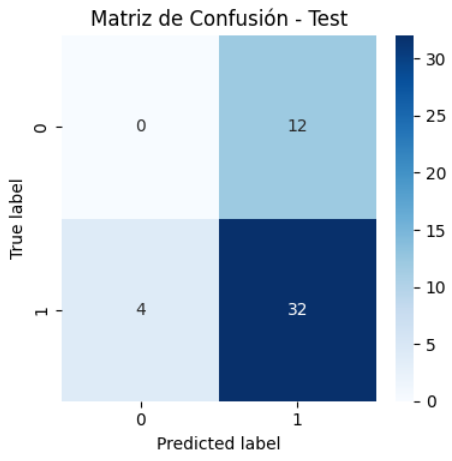
\includegraphics[width=0.35\textwidth]{images/cm_test.png}
\caption{Matriz de confusión en test (Regresión Logística)}
\label{fig:cm_test}
\end{figure}

\subsubsection{K-Nearest Neighbors } -- Evaluación en Test

En la Tabla~\ref{tab:knn_test} se presentan los resultados obtenidos por el modelo KNN en el conjunto de test. 
A pesar de un mejor balance entre precisión y recall en ambas clases (macro avg de F1-score = 0.70), se observa cierta dificultad para identificar correctamente muestras de la clase real.

\begin{table}[htbp]
\centering
\caption{Reporte de clasificación en test (KNN)}
\begin{tabular}{lcccc}
\toprule
 & Precision & Recall & F1-score & Support \\
\midrule
Real & 0.54 & 0.58 & 0.56 & 12 \\
Fake & 0.86 & 0.83 & 0.85 & 36 \\
\midrule
Accuracy & & & 0.77 & 48 \\
Macro avg & 0.70 & 0.71 & 0.70 & 48 \\
Weighted avg & 0.78 & 0.77 & 0.77 & 48 \\
\bottomrule
\end{tabular}
\label{tab:knn_test}
\end{table}

\vspace{0.2cm}
La Figura~\ref{fig:cm_knn} muestra la matriz de confusión correspondiente, destacando el comportamiento del modelo sobre ambas clases.
\begin{figure}[htbp]
\centering
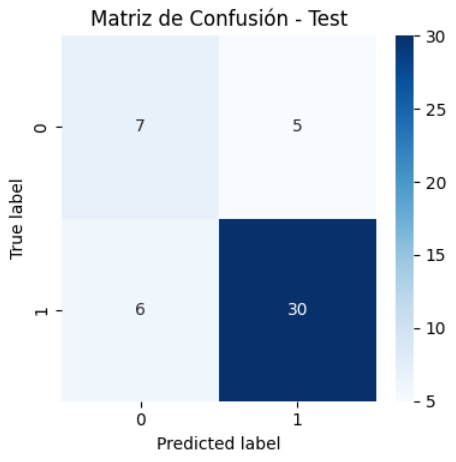
\includegraphics[width=0.35\textwidth]{images/cm_knn.png}
\caption{Matriz de confusión en test (KNN)}
\label{fig:cm_knn}
\end{figure}


\subsubsection{Random Forest }-- Evaluación en Test

La Tabla~\ref{tab:rf_test} presenta los resultados del modelo Random Forest. Se observa un mejor desempeño en la clase fake (recall=0.94), aunque limitado en la clase real (recall=0.17), obteniendo un macro avg del F1-score de 0.55.

\begin{table}[htbp]
\centering
\caption{Reporte de clasificación en test (Random Forest)}
\begin{tabular}{lcccc}
\toprule
 & Precision & Recall & F1-score & Support \\
\midrule
Real & 0.50 & 0.17 & 0.25 & 12 \\
Fake & 0.77 & 0.94 & 0.85 & 36 \\
\midrule
Accuracy & & & 0.75 & 48 \\
Macro avg & 0.64 & 0.56 & 0.55 & 48 \\
Weighted avg & 0.70 & 0.75 & 0.70 & 48 \\
\bottomrule
\end{tabular}
\label{tab:rf_test}
\end{table}

\vspace{0.2cm}
En la Figura~\ref{fig:cm_rf} se observa la matriz de confusión, donde destacan los falsos negativos de la clase real.
\begin{figure}[htbp]
\centering
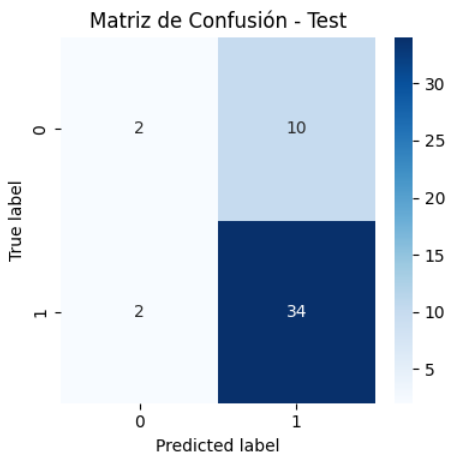
\includegraphics[width=0.35\textwidth]{images/cm_rf.png}
\caption{Matriz de confusión en test (Random Forest)}
\label{fig:cm_rf}
\end{figure}

\vspace{2cm}

\subsubsection{SVM }-- Evaluación en Test

Los resultados del modelo SVM (Tabla~\ref{tab:svm_test}) muestran un desempeño alto en la clase fake (F1=0.86) pero sin identificar correctamente ninguna muestra real, lo que reduce el macro avg del F1-score a 0.43.

\begin{table}[htbp]
\centering
\caption{Reporte de clasificación en test (SVM)}
\begin{tabular}{lcccc}
\toprule
 & Precision & Recall & F1-score & Support \\
\midrule
Real & 0.00 & 0.00 & 0.00 & 12 \\
Fake & 0.75 & 1.00 & 0.86 & 36 \\
\midrule
Accuracy & & & 0.75 & 48 \\
Macro avg & 0.38 & 0.50 & 0.43 & 48 \\
Weighted avg & 0.56 & 0.75 & 0.64 & 48 \\
\bottomrule
\end{tabular}
\label{tab:svm_test}
\end{table}

\vspace{0.2cm}
En la Figura~\ref{fig:cm_svm} se observa cómo el modelo no logra predecir correctamente la clase real.
\begin{figure}[htbp]
\centering
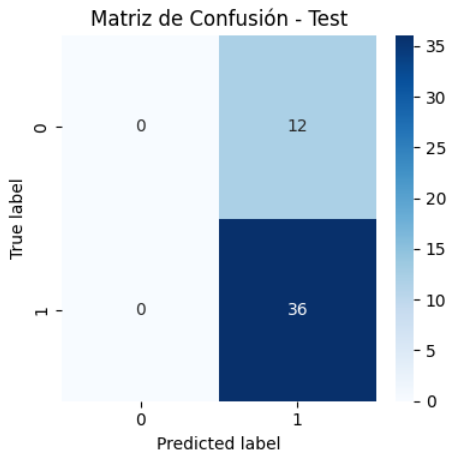
\includegraphics[width=0.35\textwidth]{images/cm_svm.png}
\caption{Matriz de confusión en test (SVM)}
\label{fig:cm_svm}
\end{figure}


\subsubsection{Red Neuronal }-- Evaluación en Test

Por último, en la Tabla~\ref{tab:nn_test} se muestran los resultados del modelo basado en red neuronal. Se aprecia un comportamiento idéntico al modelo SVM, reflejando un desequilibrio en la identificación de la clase real.

\begin{table}[htbp]
\centering
\caption{Reporte de clasificación en test (Red Neuronal)}
\begin{tabular}{lcccc}
\toprule
 & Precision & Recall & F1-score & Support \\
\midrule
Real & 0.00 & 0.00 & 0.00 & 12 \\
Fake & 0.75 & 1.00 & 0.86 & 36 \\
\midrule
Accuracy & & & 0.75 & 48 \\
Macro avg & 0.38 & 0.50 & 0.43 & 48 \\
Weighted avg & 0.56 & 0.75 & 0.64 & 48 \\
\bottomrule
\end{tabular}
\label{tab:nn_test}
\end{table}

\vspace{0.2cm}
La matriz de confusión (Figura~\ref{fig:cm_nn}) ilustra cómo todas las muestras reales fueron clasificadas erróneamente.
\begin{figure}[htbp]
\centering
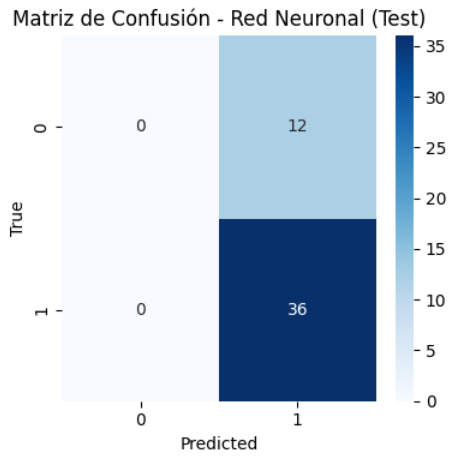
\includegraphics[width=0.35\textwidth]{images/cm_nn.png}
\caption{Matriz de confusión en test (Red Neuronal)}
\label{fig:cm_nn}
\end{figure}



\subsubsection{Análisis final}:


\begin{table}[htbp]
\centering
\caption{Comparativa de modelos en test: macro average del F1-score}
\begin{tabular}{lc}
\toprule
\textbf{Modelo} & \textbf{F1-score (macro avg)} \\
\midrule
Regresión Logística & 0.40 \\
KNN                 & 0.70 \\
Random Forest       & 0.55 \\
SVM                 & 0.43 \\
Red Neuronal        & 0.43 \\
\bottomrule
\end{tabular}
\label{tab:comparativa_f1_macro}
\end{table}


Como puede observarse en la Tabla~\ref{tab:comparativa_f1_macro}, el modelo KNN obtuvo el mejor equilibrio global entre precisión y recall de ambas clases, alcanzando un \textbf{macro average del F1-score de 0.70} y la mayor exactitud (0.77). 

Aunque Random Forest, SVM y la red neuronal obtuvieron una accuracy similar (0.75), su F1 macro avg fue inferior, principalmente debido a un desempeño más pobre sobre la clase minoritaria (imágenes reales). En contraste, la regresión logística mostró el F1 macro avg más bajo (0.40), reflejando dificultades para capturar correctamente la clase real.

Estos resultados evidencian la importancia de evaluar modelos no solo por accuracy, sino considerando métricas balanceadas como el \emph{F1 macro average}, especialmente cuando ambas clases son relevantes para la aplicación final (detectar deepfakes sin penalizar excesivamente la clase real). 






\section{Conclusiones}

En este trabajo se exploró el problema de detección de deepfakes mediante la extracción de características manuales (GLCM, LBP, entre otras) y la aplicación de modelos tradicionales de aprendizaje automático. 

Se identificaron varias limitaciones relevantes. En primer lugar, las \emph{features} extraídas no resultaron ser las más representativas o discriminativas para el problema, afectando así la capacidad de los modelos para generalizar, especialmente sobre la clase real. Además, los modelos tradicionales de aprendizaje supervisado, como regresión logística, SVM o Random Forest, mostraron un rendimiento limitado, reflejado en valores de \emph{F1-score macro average} relativamente bajos en comparación con lo esperado para un sistema robusto de detección.

Tal como se evidencia en la literatura revisada, la naturaleza compleja y matizada de los deepfakes requiere recurrir a enfoques más avanzados, como redes neuronales convolucionales profundas o modelos basados en aprendizaje transferido, que han demostrado un desempeño superior al poder aprender representaciones jerárquicas directamente de los datos en crudo. 

Finalmente, este trabajo resalta la importancia de considerar tanto el \emph{recall} como la \emph{precisión} de ambas clases, utilizando métricas balanceadas como el \emph{F1-score macro average}, especialmente en contextos donde los falsos positivos y falsos negativos pueden tener implicaciones significativas.

 Finalmente, este proyecto evidencia que, aunque no siempre se obtienen los resultados esperados, el proceso de diseño, prueba y validación de modelos aporta un aprendizaje valioso, y que el trabajo en equipo y la reflexión crítica son clave para identificar limitaciones y proponer mejoras futuras.
















\bibliographystyle{IEEEtran}
\bibliography{referencias}


\end{document}
